\documentclass[border=1mm]{standalone}

\usepackage{listings}
\usepackage{tikz}
\usetikzlibrary{positioning,calc}
\usetikzlibrary{fit,backgrounds}
\usetikzlibrary{shapes.multipart}
\pgfsetlayers{background,cpu,main}

\pgfdeclarelayer{background}
\pgfdeclarelayer{cpu}
\pgfdeclarelayer{main}

\newsavebox\mybox

\lstset{language=Python}

\usepackage{fontawesome5}

\begin{document}


\begin{tikzpicture}

   \tikzstyle{k}=[draw,fill=green!20,font=\ttfamily,node distance=18mm]
   \tikzstyle{v}=[font=\LARGE] 
   \tikzstyle{s}=[draw,rounded corners,on background layer]

   \node (k1) [k] { "Ola Nordmann" } ;
   \node (k2) [k,below=of k1,xshift=-12mm,yshift=5mm] { "Kari Nordmann" } ;
   \node (k3) [k,below=of k2,xshift=7mm,] { "John Smith" } ;
   \node (k4) [k,below=of k3,yshift=-3mm,xshift=-8mm] { "Jane Doe" } ;


   \node (v1) [v,right=of k1] {\faAddressCard } ;
   \node (v2) [v,below=of v1] {\faAddressCard } ;
   \node (v3) [v,below=of v2] {\faAddressCard } ;
   \node (vx) [v,below=of v3] {$\vdots$} ;
   \node (v4) [v,below=of vx] {\faAddressCard } ;

   \begin{scope}[on background layer]
   \node (k) [s,fill=green!50,fit=(k1) (k2) (k4)] {} ;
   \node (v) [s,fill=yellow!10,fit=(v1) (v4)] {} ;
   \end{scope}

   \path [draw,->] (k1) -- (v1) ;
   \path [draw,->] (k2) -- (v2) ;
   \path [draw,->] (k3) -- (v3) ;
   \path [draw,->] (k4) -- (v4) ;

\end{tikzpicture}

\end{document}

